\documentclass[14pt]{beamer}
\usetheme{Malmoe}
\usepackage[utf8]{inputenc}
\usepackage{amsmath}
\usepackage{amsfonts}
\usepackage{amssymb}
\usepackage{graphicx}
\usepackage{multicol}
\author{Scott Atherley, Clarence Dillon, Vince Kane}
\title{A Model of Policy Formation through Simulated Annealing}
%\setbeamercovered{transparent} 
%\setbeamertemplate{navigation symbols}{} 
\logo{} 
\institute{George Mason University} 
\date{1 April 2015} 
\subject{Social Behavioral and Predictive Modeling Conference 2015} 
\begin{document}

% slide 0
\begin{frame}
\titlepage
\end{frame}

% slide 1
\section*{Introduction}
\begin{frame}{Introduction}
\begin{itemize}
\item Why was the $113^{th}$ U.S. Congress so unproductive?
\item Do diversity and policy divides result in deadlock and dissatisfaction?
\end{itemize}

\begin{block}{Traditional Modeling}
  Congressional voting reflects ideology, influences and committee dynamics.
   \end{block}
\end{frame}

% slide 2
\begin{frame}{Our Contribution}
\begin{itemize}
\item General model, broadly applicable to complex behaviors of policy-making organizations
\item Computational model of policy development in which ideology is arbitrary
\item The process optimizes satisfaction within a system of competing preferences

\begin{block}{Simulated Annealing}
  Non-deterministic method to fit proposals to preferences
   \end{block}
\end{itemize}
\end{frame}

% slide 3
\section*{Method} %section 2
\begin{frame}{Model and its Cases}
\begin{itemize}
\item A model of policy formation through simulated annealing
\item Each `session' is a unique mix of legislators; new network
 \begin{itemize}
 \item a legislator proposes a solution to an issue
 \item others append positions on other issues to make the draft favorable
 \item once among peers and again in committee
 \item final vote 
 \end{itemize}  
\item We measure productivity, satisfaction, \textit{etc} at the session level
\end{itemize}
\end{frame}

%\subsection*{Overview} %section 2.1
% slide 4
\subsection*{Initialization} % section 2.2
\begin{frame}{Initialization}
\begin{itemize}
\item Generate a \texttt{State} object to hold scenario parameters 
\item Includes 100 heterogeneous legislators
\item Organizes legislators into a network, committees
\item Party and state priorities are set
\end{itemize}
\end{frame}

% slide 5
\begin{frame}{Model Environment}%section 2.2.1
\begin{itemize}
\item Party ``platforms'' are positions and priorities of key issues
 \begin{itemize}
 \item includes and state-level priorities
 \item random sample of other issues
 \end{itemize}
\item Platforms are seeds for stochastic generation of legislator preferences  
\end{itemize}
\end{frame}

% slide 6
\begin{frame}{Legislators} %section 2.2.2
\begin{itemize}
\item Legislator issue priorities assigned with stochastic preference to state seed values
 \begin{itemize}
 \item Power-law distributed priority set for each legislator
 \item Have one of $2^4 = 16$ possible positions on each issue
 \end{itemize}
\item Creates heterogeneous set of legislator agents with correlated issue priorities within a party  
\end{itemize}
\end{frame}

% slide 7; two cols for text and colorized network plots
\begin{frame}{Network} %section 2.2.3
\begin{columns}[T] %aligned to top
\begin{column}[T]{9cm} 
\begin{itemize}
\item Final step: legislators networked through homophily, preferential attachment (PA) 
 \begin{itemize}
 \item PA $m=5$ new edges randomly selected from \textit{pdf} from potential allies
 \item Preference-weighted likelihood over all issues
 \end{itemize}
\item Produces ``small world'' network, like Congress 
\end{itemize}
\end{column}
\begin{column}[T]{3.5cm}
 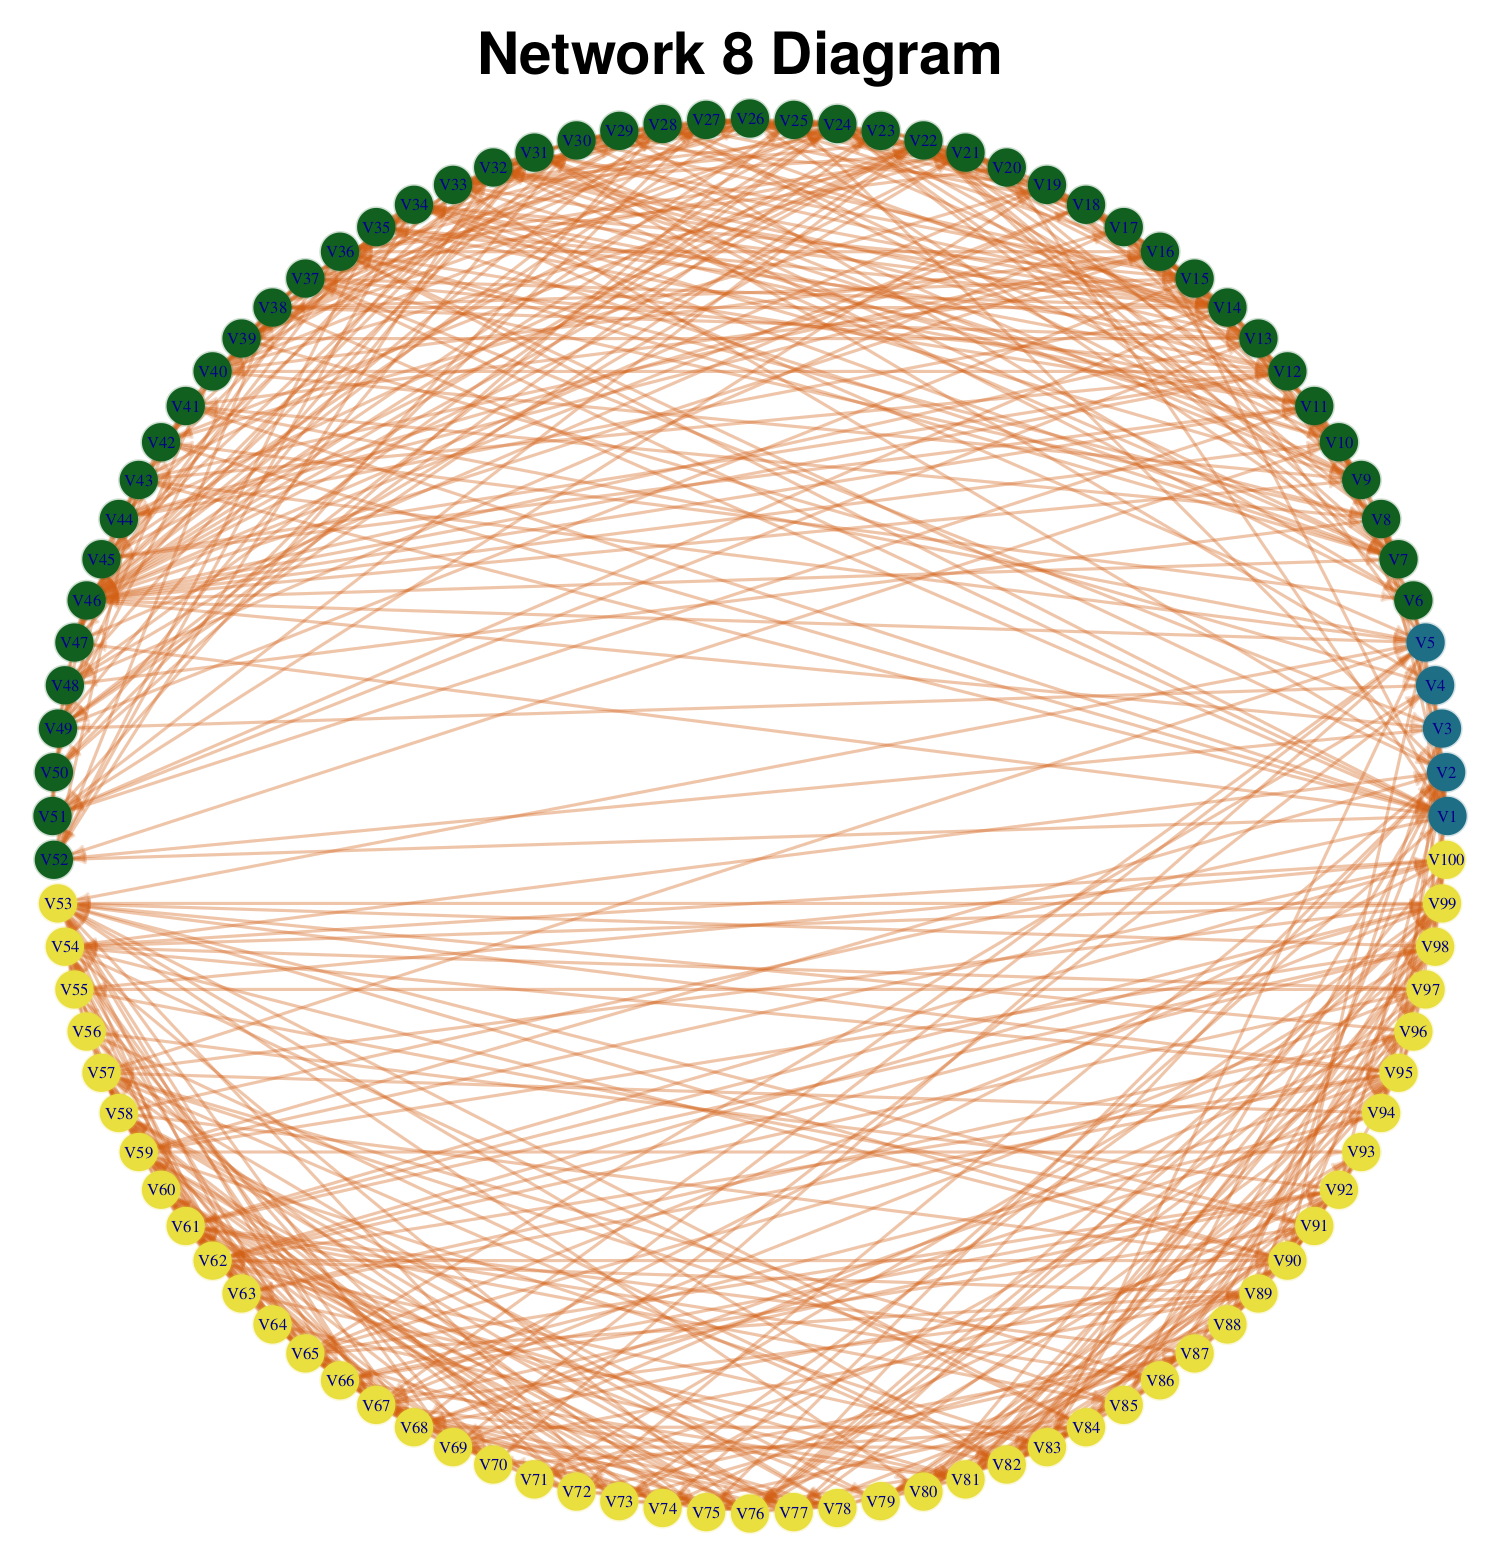
\includegraphics[width=3.45cm]{sbp_network_diagram_2014-05-03_170445_crop.png}
 \label{One example of the 72 networks produced in the simulation baseline data.}
\end{column}
\end{columns}

\end{frame}

% slide 8
\subsection*{Simulation Algorithm} % section 2.3

\begin{frame}{Simulation}
\begin{itemize}
\item Legislators begin to legislate
\item Up to 200 proposals for each session
\item Session stops if all 75 issues pass   
\end{itemize}
\end{frame}

\begin{frame}{Proposal} %section 2.3.1
\begin{itemize}
\item Random legislator selected 
\item Proposes a draft with their position on any issue not passed into law
\end{itemize}
\end{frame}


\begin{frame}{Draft Circulation} %section 2.3.2
\begin{itemize}
\item Peers (first-order connections) co-sponsor the bill
\item Co-sponsors revise the draft via SA
 \begin{itemize}
 \item may add issues
 \item may revise positions
 \end{itemize}   
\end{itemize}
\end{frame}


\begin{frame}{Committee Review} %section 2.3.3
\begin{itemize}
\item Draft goes to committee
\item Legislators with core issue as high-priority makeup the committee
\item Committee revises sponsored draft via SA (same rules)
\end{itemize}
\end{frame}


\begin{frame}{Floor Vote} % section 2.3.4
\begin{itemize}
\item Bill referred to floor
\item Legislators vote `yes' if their satisfaction  
\item Simple majority passes bill into law 
 \begin{itemize}
 \item issue removed from future work
 \item model logs statistics for analysis
 \end{itemize}
\end{itemize}
\end{frame}


\begin{frame}{Simulated Annealing} %section 2.3.5
\begin{itemize}
\item Implemented as Metropolis algorithm
\item Energy is the cumulative dissatisfaction of all reviewers, over all dimensions
\item Dissatisfaction increases of 0.1 accepted with 50\% probability at max temperature
\item Higher satisfaction energy states accepted automatically
\end{itemize}
\end{frame}


\subsection*{Model Calibration} % section 2.4
\begin{frame}{Calibration}
\begin{itemize}
\item Calibrated primarily with \texttt{satisfaction\_threashold} parameter
\item Adjusted to match real-world ~4\%, average in recent history
\end{itemize}
\end{frame}


\subsection*{Experiments} % section 2.5
\begin{frame}{Experiments}

\begin{table}[htp]
\tiny
 \caption{Simulation Parameter Space}
 \begin{tabular}{lp{2.17in}c}
 \hline\noalign{\smallskip}
 Parameter & Description & Value [Variation] \\
 \noalign{\smallskip}
 \hline
 \noalign{\smallskip}
 \texttt{Unaffilitated\_Fraction} & Fraction of the legislative population with no ideological party  affiliation. & [0.05, 0.5, 1.0] \\
 \texttt{Green\_Fraction} & Fraction of the party-affiliated population belonging to the \textit{Green} party. Remainder belong to the Yellow party. & [0.5, 0.75, 1.0] \\
 \texttt{Ideology\_Issues} & Ideological platform issues for the parties. & [0, 5] \\
 \texttt{State\_Priorities} & High-priority issues for all legislators, regardless of affiliation. & [0, 5] \\
 \hline
 \end{tabular}
 \label{params}
\end{table}

\begin{itemize}
\item 28 unique experiment combinations
\item 30 simulations per experiment 
\end{itemize}
\end{frame}


\section*{Results and Findings} % section 3

\subsection*{Results} % section 
\begin{frame}{Results}
\begin{block}{On dysfunction:}
  Fourteen of 28 cases produced \textbf{NO} laws
   \end{block}

\begin{itemize}
\item All four cases with no party structure
\item Scenarios with 50\% unaffiliated, 25\% Green, 25\% Yellow
\item Scenarios with no external priorities
\item One other case with 5\% unaffiliated, 50\% Green and no ideology-based priorities  
\end{itemize}
\end{frame}

\subsection*{Findings}

\begin{frame}
 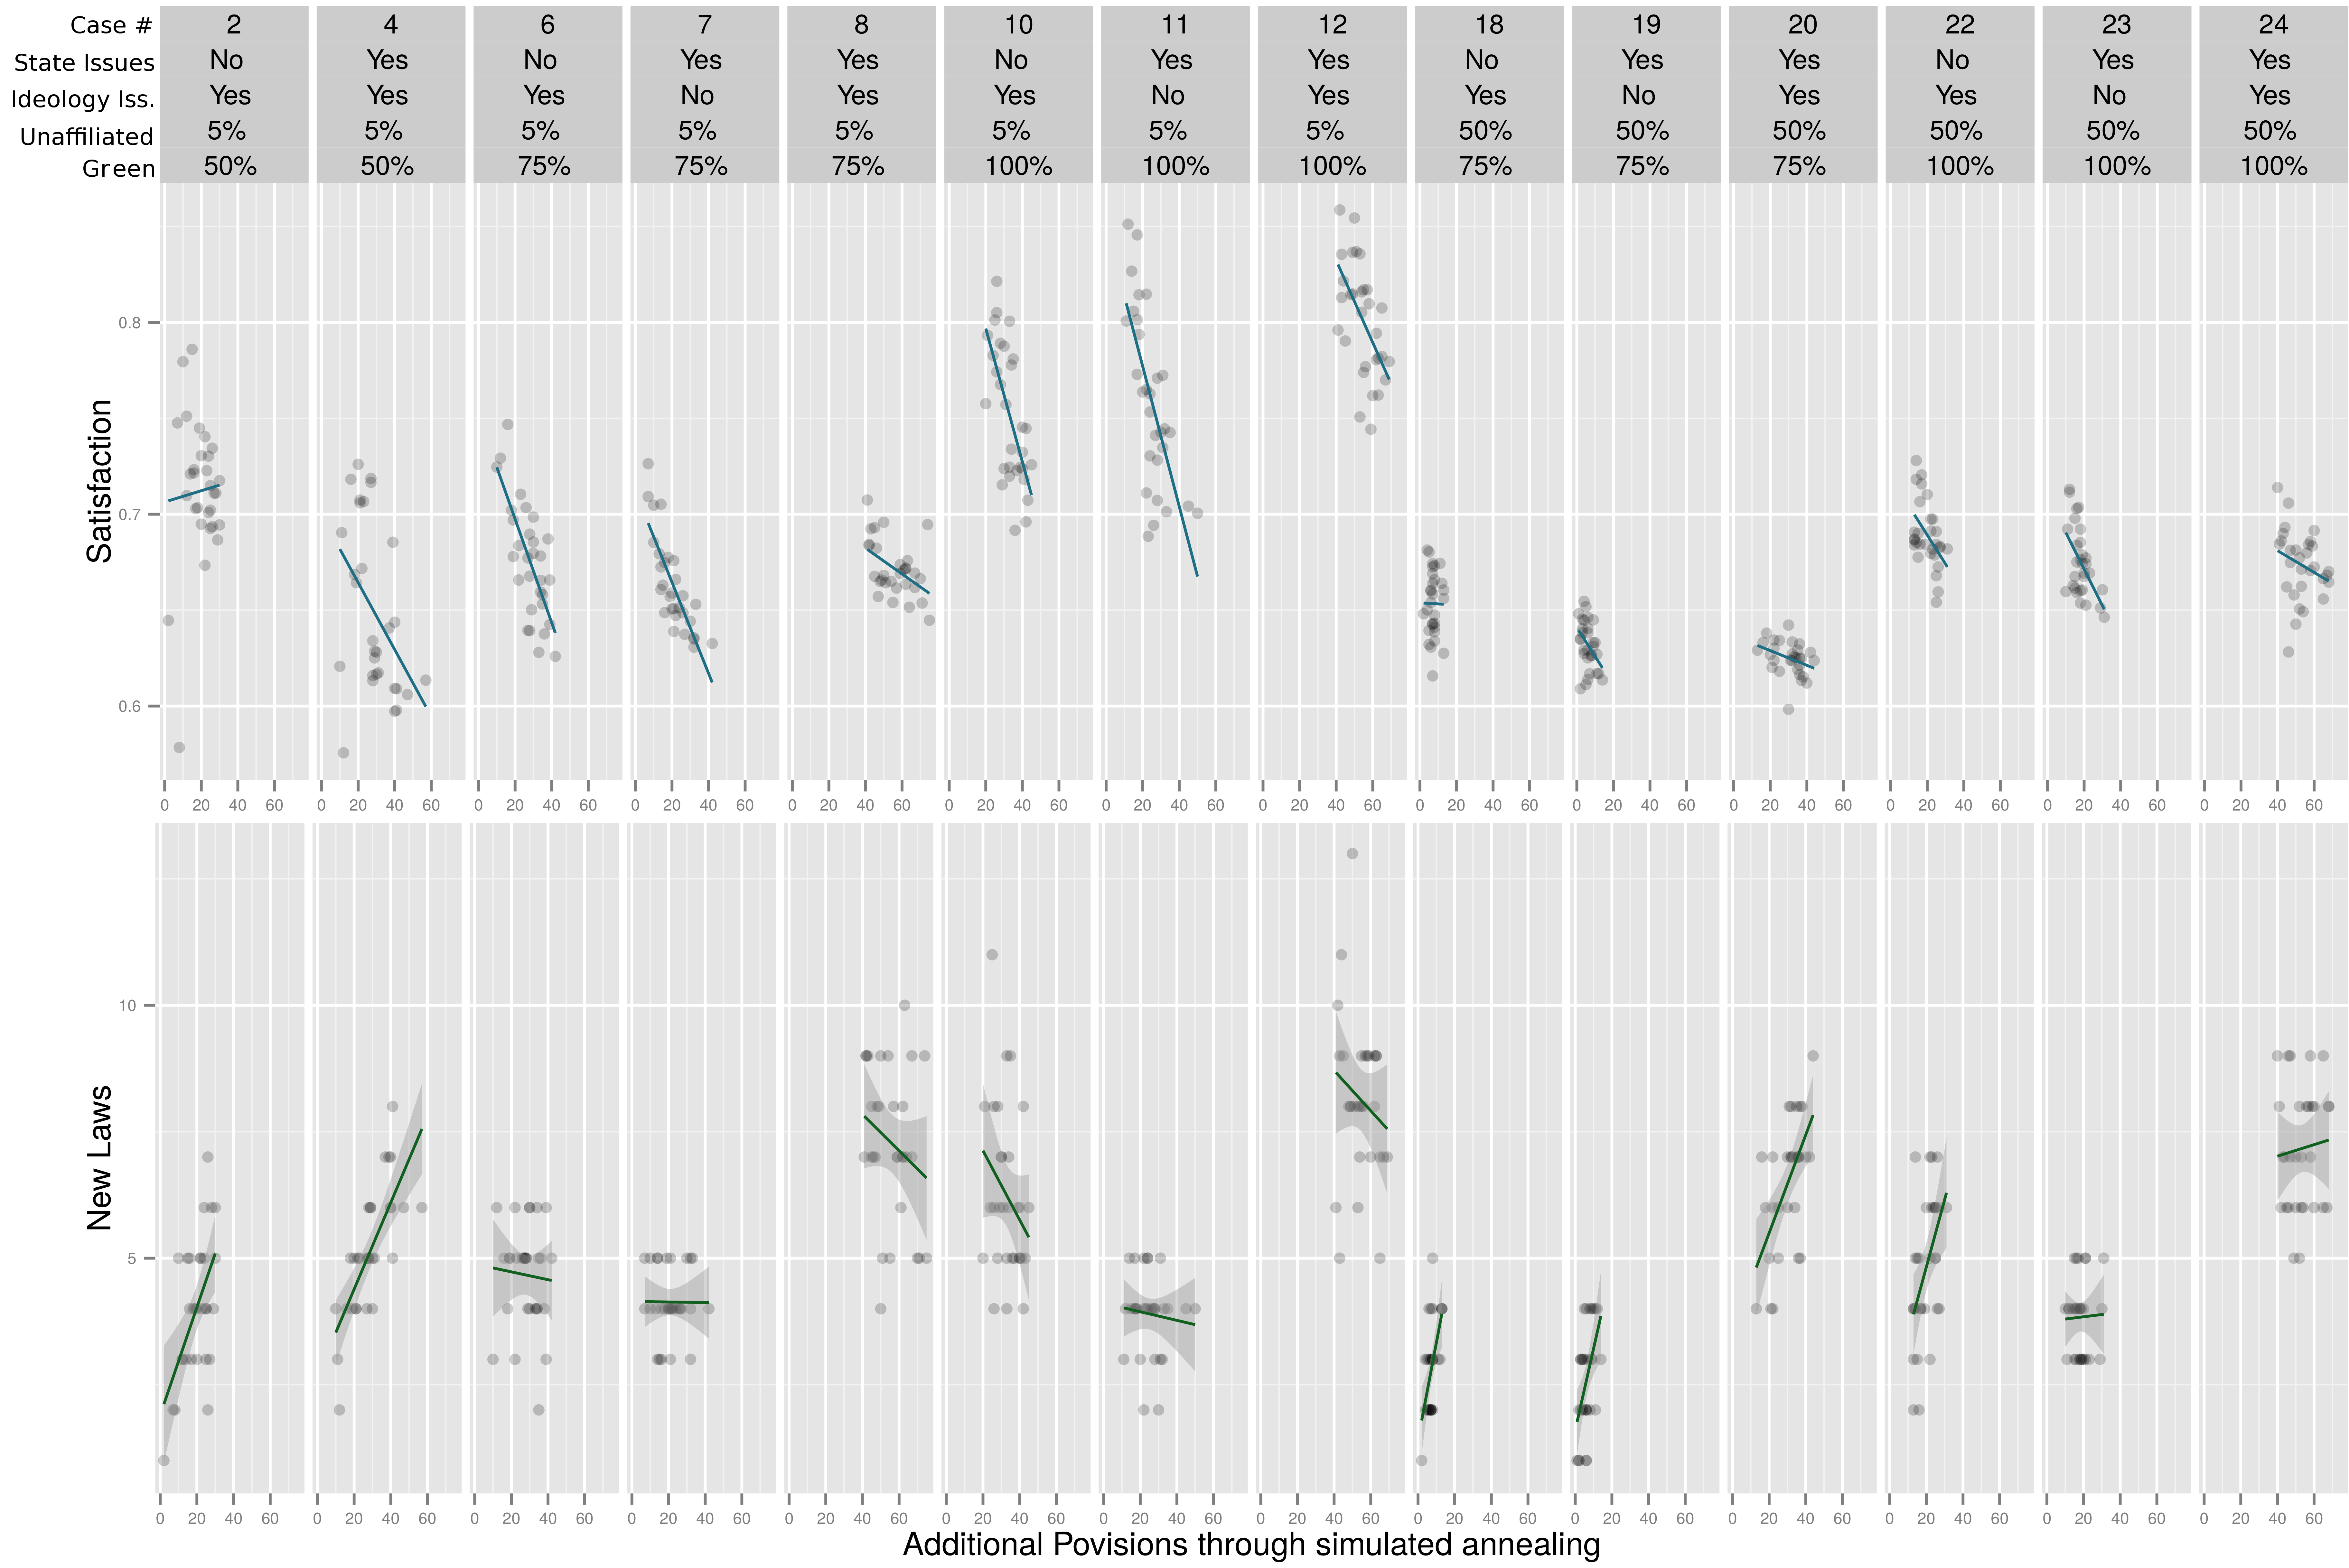
\includegraphics[width=10.8cm]{combinedResults_newColors.png}
 %\label{One example of the 72 networks produced in the simulation baseline data.}
\end{frame}



\begin{frame}{Findings}
\begin{block}{Finding \#1}
  Higher correlation of preferences results in higher productivity.
\end{block}
\begin{block} {Evidence}
  Compare cases 6 and 7 to cases 8, 10 and 12, for example.
\end{block}
\end{frame}


\begin{frame}{Findings}
\begin{block}{Finding \#2}
  Higher productivity requires increased number of additional provisions.
\end{block}
\begin{block} {Evidence}
  Nine of 14 cases show positive correlation; 3 others show high threshold minimum.
\end{block}
\end{frame}
 
 
\begin{frame}{Findings}
\begin{block}{Finding  \#3}
  Partisanship is not necessarily an impediment to productivity.   
\end{block}
\begin{block}{Evidence}
  See cases 2 and 4.
\end{block}
\end{frame}


\begin{frame}{Findings}
\begin{block}{Finding  \#4}
  Bipartisan networks (even division of party-affiliated legislators) with more external priorities can be more productive than majorities or super-majorities with fewer external priorities.
\end{block}
\begin{block}{Evidence}
  Compare cases 4 to cases 11, 18, 19, and 28.
\end{block}
\end{frame}

\begin{frame}{Findings}
\begin{block}{Finding \#5}
  Overall satisfaction decreases with increases number of additional provisions, but productivity is higher.  
\end{block}
\begin{block}{Evidence}
  Cases 4, 7, 18, 19, 20, 22, 23, and 24. 
\end{block}
\end{frame}

\begin{frame}
 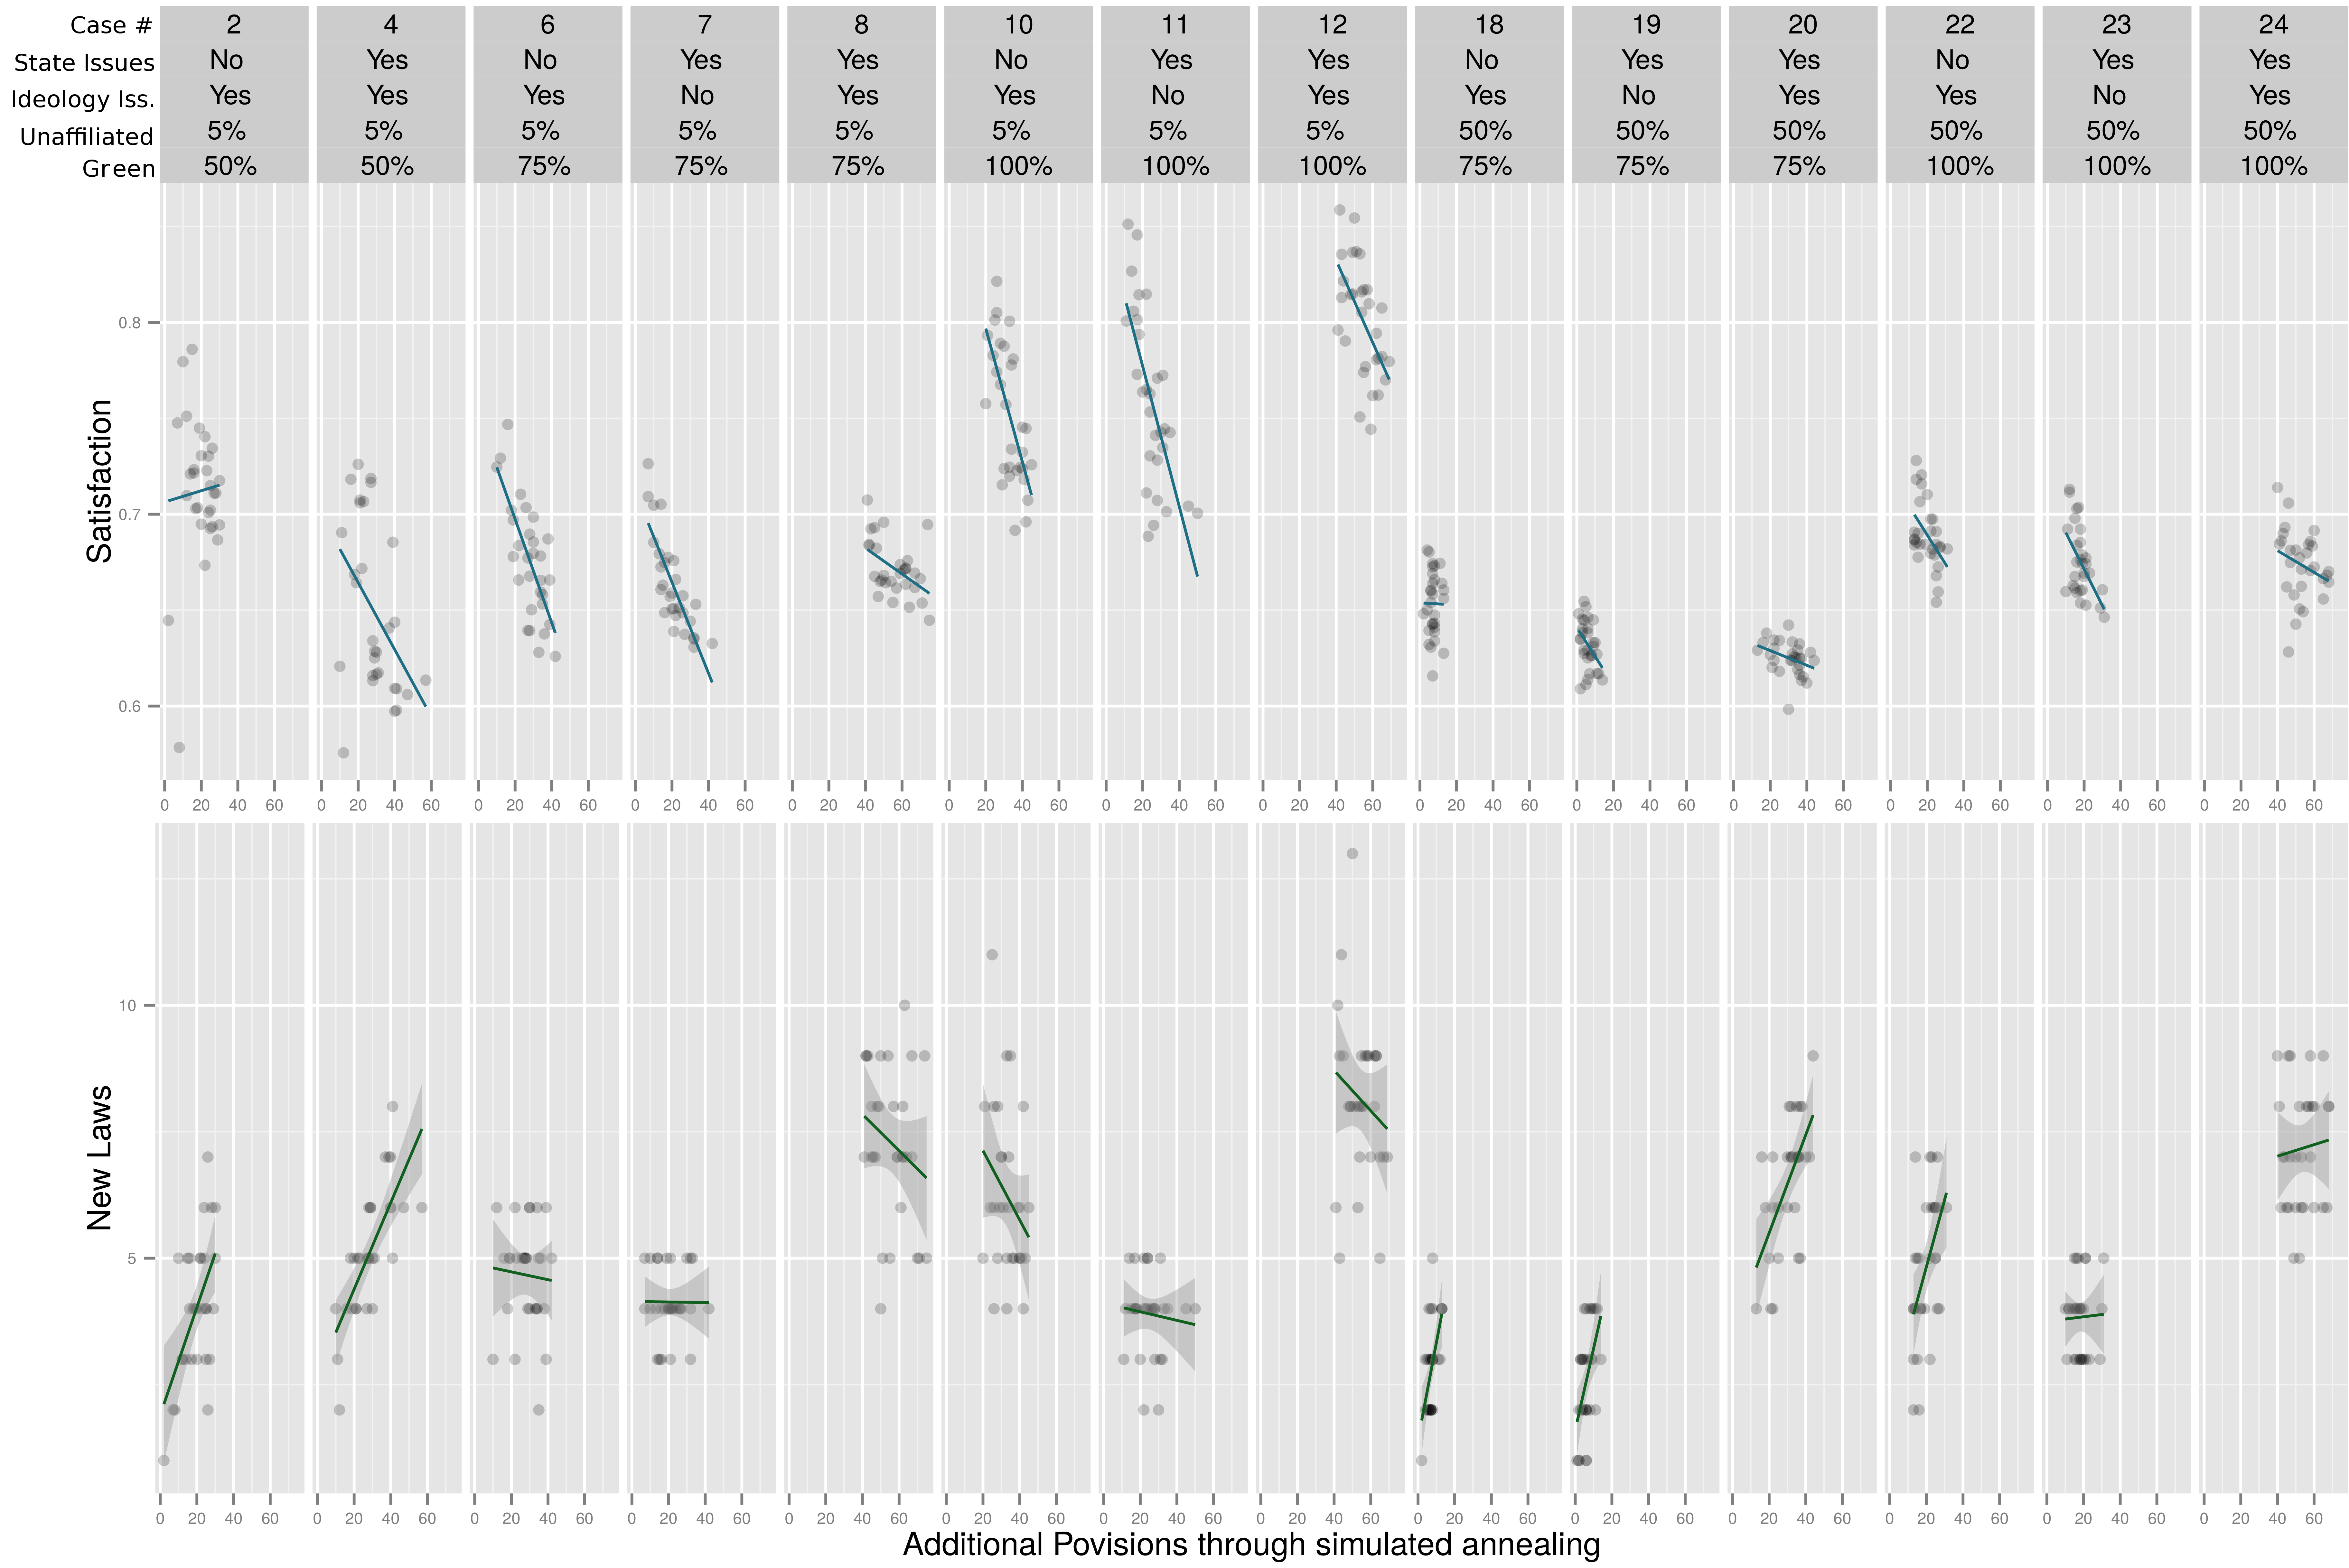
\includegraphics[width=10.8cm]{combinedResults_newColors.png}
 %\label{One example of the 72 networks produced in the simulation baseline data.}
\end{frame}


\section*{Discussion} % section 4

\begin{frame}{Discussion}
\begin{itemize}
\item Externally-defined priorities 
\item Impact of polarization
\item Efficiency vs productivity and the additional provisions
\item More provisions reduces satisfaction 
\end{itemize}
\end{frame}


\begin{frame}{External Priorities}
\begin{itemize}
\item Having external priorities is important for productivity
 \begin{itemize}
 \item The more, the better (observed in our experiments)
 \item Absence of external priorities correlates with no productivity
 \end{itemize}
\item  Future research should look at role of leadership 
\end{itemize}
\end{frame}

\begin{frame}{Polarization}
\begin{itemize}
\item We expected evidence that polarization reduces productivity and satisfaction
 \begin{itemize}
 \item Findings \#3 and \#4 do not support this hypothesis
 \item Dysfunction of the $113^{th}$ U.S. Congress may be caused by something else
 \end{itemize}
\end{itemize}
\end{frame}

\begin{frame}{Productivity}
\begin{itemize}
\item Riders on bills is the ``cost of doing business''
 \begin{itemize}
 \item Can increase productivity
 \item Usually decrease satisfaction
 \end{itemize}
\item Also decreases system efficiency 
\end{itemize}
\end{frame}

\begin{frame}{Satisfaction}
\begin{itemize}
\item Compromise leads to minimum of satisfaction
 \begin{itemize}
 \item Perhaps some bills start off with low satisfaction and add provisions to garner votes?
 \item How much of a majority is required to overcome dissatisfaction levels?
 \end{itemize}
\item Can leadership intervention overcome unproductive structures? (ideology or priorities?) 
\end{itemize}
\end{frame}

\subsection*{} % section 4.1
\begin{frame}{Implications for Future Research}
\begin{itemize}
\item Network structures and characteristics
 \begin{itemize}
 \item Experiment with finer resolutions to find tipping points in system behaviors
 \item Can we find thresholds that produce both productivity and satisfaction?
 \end{itemize}
\item External priorities
  \begin{itemize}
  \item How much leadership intervention will overcome unproductive structures?
  \item How many state priorities are required to ensure preference correlation?
  \end{itemize}
\end{itemize}
\end{frame}


\section*{Summary} % section 5
\begin{frame}{Summary}
\begin{itemize}
\item We modeled policy-making with SA as complex problem with interdependent constraints
 \begin{itemize}
 \item Case study: U.S Congress legislation process
 \item Method is applicable to other social processes
 \end{itemize}
\item Partisanship 
 \begin{itemize}
 \item Alone, does not impede productivity and satisfaction 
 \item Overcome with priority and preference alignment
 \end{itemize}
\item Simulated Annealing
 \begin{itemize} 
 \item Useful to model policy-making computationally
 \item Recommended for other research
 \end{itemize}
\end{itemize} 
\end{frame}

%\section*{References} % Not numbered

\end{document}